\documentclass[a4paper,12pt]{report}

\usepackage[utf8]{inputenc}
\usepackage{graphicx}
\usepackage{float}
\usepackage{hyperref}
\usepackage{longtable}
\usepackage{array} 
\usepackage{booktabs}
\usepackage[inkscapelatex=false]{svg}
\usepackage{tabularx}

\usepackage[italian]{babel}

\title{
	Smart Tank Monitoring System\\
	\large Anno Accademico 2025-2026
}

\author {
	Autori:\\Davide Mancini\\Filippo Ricciotti\\Martina Malagoli
}

\begin{document}

\maketitle

\newpage

\tableofcontents

\chapter{Introduzione}

\section{Obiettivo}

L'obiettivo del progetto è creare un'infrastruttura per monitorare e regolare automaticamente il livello dell'acqua piovana raccolta in una cisterna, aprendo o chiudendo un canale di scarico in base a quanto sta salendo il livello.\\
Il sistema è stato considerato nei suoi quattro sottosistemi:
\begin{itemize}
     \item Il \textbf{TMS} (Tank Monitoring Subsystem) gira su un ESP32 e si occupa solo di leggere il livello dell'acqua tramite un sensore sonar, pubblicandolo poi via MQTT.
    \item Il \textbf{WCS} (Water Channel Subsystem), su Arduino UNO, muove fisicamente la valvola tramite un servomotore, sia quando riceve un comando dal CUS sia quando l'operatore la controlla a mano con un potenziometro.
    \item Il \textbf{CUS} (Control Unit Subsystem) è il cervello del sistema: un'applicazione Java che riceve i dati dal TMS, decide come deve comportarsi la valvola e tiene aggiornati sia il WCS che la dashboard.
    \item Il \textbf{DBS} (Dashboard Subsystem) è una semplice pagina web che mostra lo stato del sistema e permette di cambiare modalità o regolare la valvola da remoto.
\end{itemize}

\section{Componenti utilizzati}
\subsection{TMS - ESP32}
\begin{table}[H]
	\centering
	\begin{tabular}{|l|l|c|l|}
		\hline
		\textbf{Componente} & \textbf{Modello} & \textbf{Pin} & \textbf{Interfaccia} \\
		\hline
		Sensore sonar TRIG & HC-SR04 & 32 & Output \\
		\hline
		Sensore sonar ECHO & HC-SR04 & 34 & Input \\
		\hline
		LED verde & Standard & 14 & Output \\
		\hline
		LED rosso & Standard & 25 & Output \\
		\hline
	\end{tabular}
	\caption{Componenti hardware del TMS}
\end{table}

\begin{figure}[H]
	\centering
	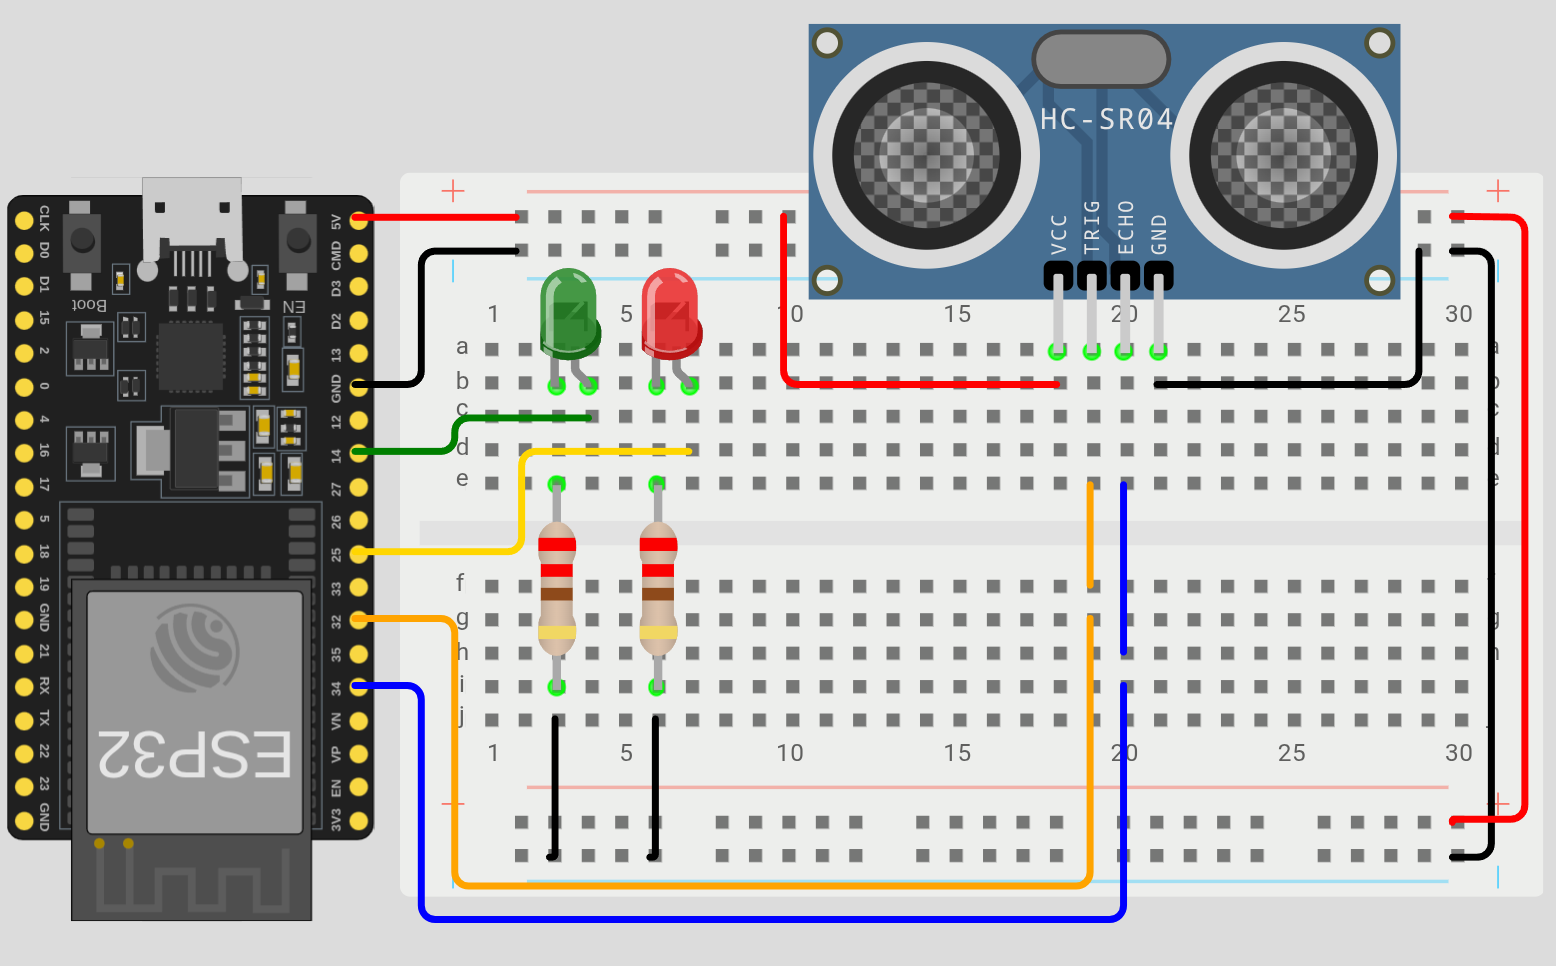
\includegraphics[width=1\textwidth]{images/tms_breadboard.png}
	\caption{Schema di collegamento del TMS}
	\label{fig:tms-breadboard}
\end{figure}

\newpage

\subsection{WCS - Arduino}
\begin{table}[H]
	\centering
	\begin{tabular}{|l|l|c|l|}
		\hline
		\textbf{Componente} & \textbf{Modello} & \textbf{Pin} & \textbf{Interfaccia} \\
		\hline
		Bottone & Standard & 4 & Input \\
		\hline
		Potenziometro & Standard & A0 & Analog \\
		\hline
		Servo motore & SG90 & 9 & PWM \\
		\hline
		Display LCD I2C & 16x2, indirizzo 0x27 & A4/A5 & I2C \\
		\hline
	\end{tabular}
	\caption{Componenti hardware del WCS}
\end{table}

\begin{figure}[H]
	\centering
	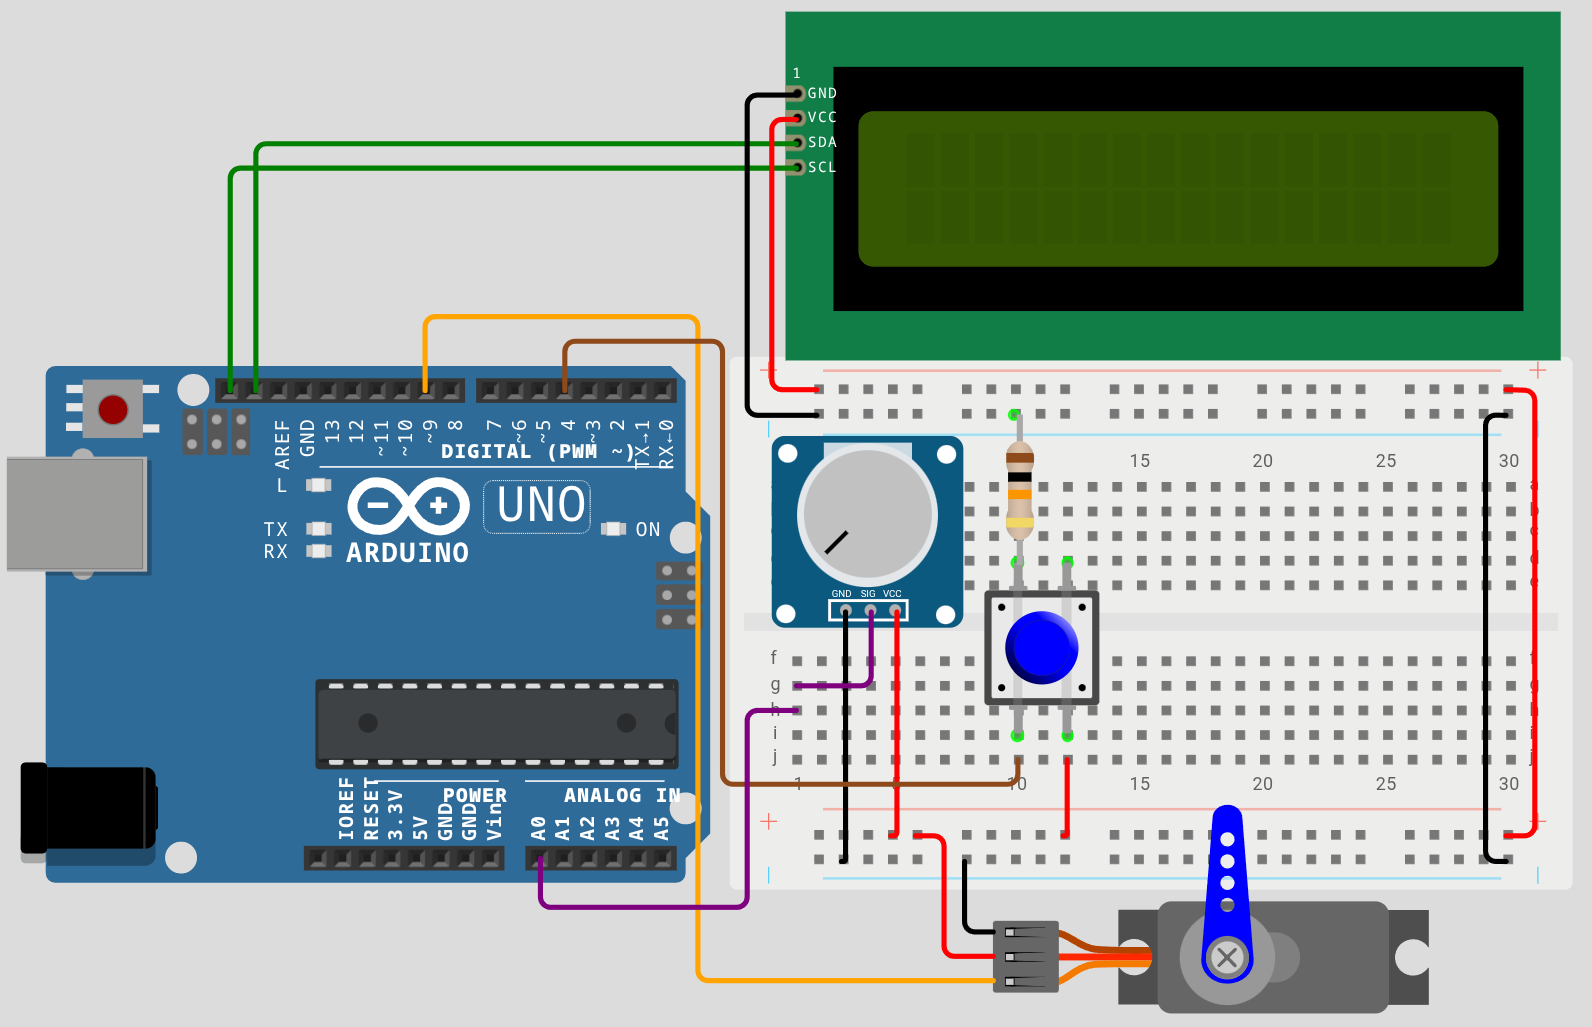
\includegraphics[width=1\textwidth]{images/wcs_breadboard.png}
	\caption{Schema di collegamento del WCS}
	\label{fig:wcs-breadboard}
\end{figure}

\chapter{Architettura del Software}



\section{TMS (ESP32)}
Il firmware del TMS è organizzato in task su FreeRTOS, ciascuna con un compito isolato:

\begin{itemize}
	\item \textbf{SonarTask} legge periodicamente il sensore e scrive il livello misurato nel \texttt{Context} condiviso.
	\item \textbf{MqttTask} tiene viva la connessione al broker, controlla lo stato della rete e pubblica un nuovo valore ogni volta che \texttt{SonarTask} ne produce uno.
	\item \textbf{LedTask} guarda semplicemente lo stato di rete riportato da \texttt{MqttTask} e decide quale dei due LED accendere: è di fatto una piccola macchina a stati a due soli stati, rete OK e problema di rete.
\end{itemize}
\begin{figure}[H]
	\centering
	\includesvg[width=0.55\textwidth]{images/LedTask.svg}
	\caption{Macchina a stati di \texttt{LedTask}}
	\label{fig:tms-ledtask}
\end{figure}
\newpage

\section{WCS (Arduino)}
Sul WCS è stato adottato un executive ciclico, basato su un timer hardware e uno scheduler che fa girare le task a periodi fissi:
\begin{itemize}
	\item \textbf{SerialCommTask} legge e scrive i messaggi sulla seriale verso il CUS, secondo il protocollo descritto più avanti.
	\item \textbf{ModalityTask} gestisce il cambio tra \texttt{AUTOMATIC} e \texttt{MANUAL} quando viene premuto il pulsante, con debounce per evitare toggle multipli su una singola pressione.
	\item \textbf{PotentiometerTask} legge il potenziometro quando si è in \texttt{MANUAL}, con una deadband per evitare che sovrascriva il valore ricevuto da altri subsystem con il rumore del sensore.
	\item \textbf{ValveTask} è una macchina a stati con solo due stati (\texttt{IDLE} e \texttt{MOVING}) che sposta il servo verso il target a velocità costante, calcolando ad ogni tick lo spostamento in base al tempo realmente trascorso.
	\item \textbf{LCDTask} mostra sul display l'apertura corrente della valvola e la modalità in cui si trova il sistema, incluso lo stato \texttt{UNCONNECTED}.
\end{itemize}
\begin{figure}[H]
	\centering
	\includesvg[width=0.8\textwidth]{images/ValveTask.svg}
	\caption{Macchina a stati di \texttt{ValveTask}}
	\label{fig:wcs-valvetask}
\end{figure}

\newpage

\section{CUS (Java)}
Il CUS è un'applicazione Java che si appoggia a Eclipse Paho per il client MQTT, a JSSC per la seriale e a Vert.x per il server HTTP verso il DBS. È composto da:
\begin{itemize}
	\item \textbf{MqttListener}, che riceve i messaggi del livello dell'acqua dal TMS e li passa alla policy.
	\item \textbf{TankPolicy}, il componente che decide l'apertura della valvola quando in modalità \texttt{AUTOMATIC}:\\
	 una macchina a stati con quattro stati (\texttt{CLOSED}, \texttt{WAITING\_T1}, \texttt{HALF\_OPEN}, \texttt{FULL\_OPEN}) che tiene conto delle soglie L1 e L2 e del tempo T1 richiesto prima di aprire parzialmente la valvola.
	\item \textbf{ConnectionWatchdog}, che tiene traccia di quanto tempo è passato dall'ultimo dato ricevuto dal TMS e fa scattare lo stato \texttt{UNCONNECTED} superato il tempo T2.
	\item \textbf{SerialService}, che parla con il WCS sullo stesso protocollo a righe descritto più avanti.
	\item \textbf{HttpApiServer}, che espone l'endpoint consumato dal DBS.
	\item \textbf{MainFrame}, un'interfaccia Swing che permette di vedere lo stato del sistema direttamente dal PC su cui gira il CUS.
\end{itemize}
\begin{figure}[H]
	\centering
	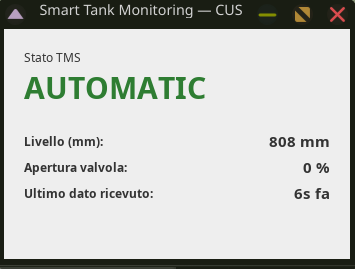
\includegraphics[width=0.67\textwidth]{images/cus.png}
	\caption{GUI del \texttt{CUS}}
	\label{fig:cus-gui}
\end{figure}

\begin{figure}[H]
	\centering
	\includesvg[width=1\textwidth]{images/TankPolicy.svg}
	\caption{Macchina a stati di \texttt{TankPolicy}}
	\label{fig:cus-tankpolicy}
\end{figure}

\newpage 

\section{DBS - Dashboard Subsystem}
Il DBS è scritto in HTML, CSS e JavaScript puro, senza framework, con Chart.js per disegnare il grafico dello storico dei livelli. Comunica col CUS tramite \texttt{fetch()}: fa polling periodico su \texttt{GET /api/data} per restare aggiornato, e invia i comandi dell'operatore con \texttt{POST /api/data}.

\begin{figure}[H]
	\centering{}
	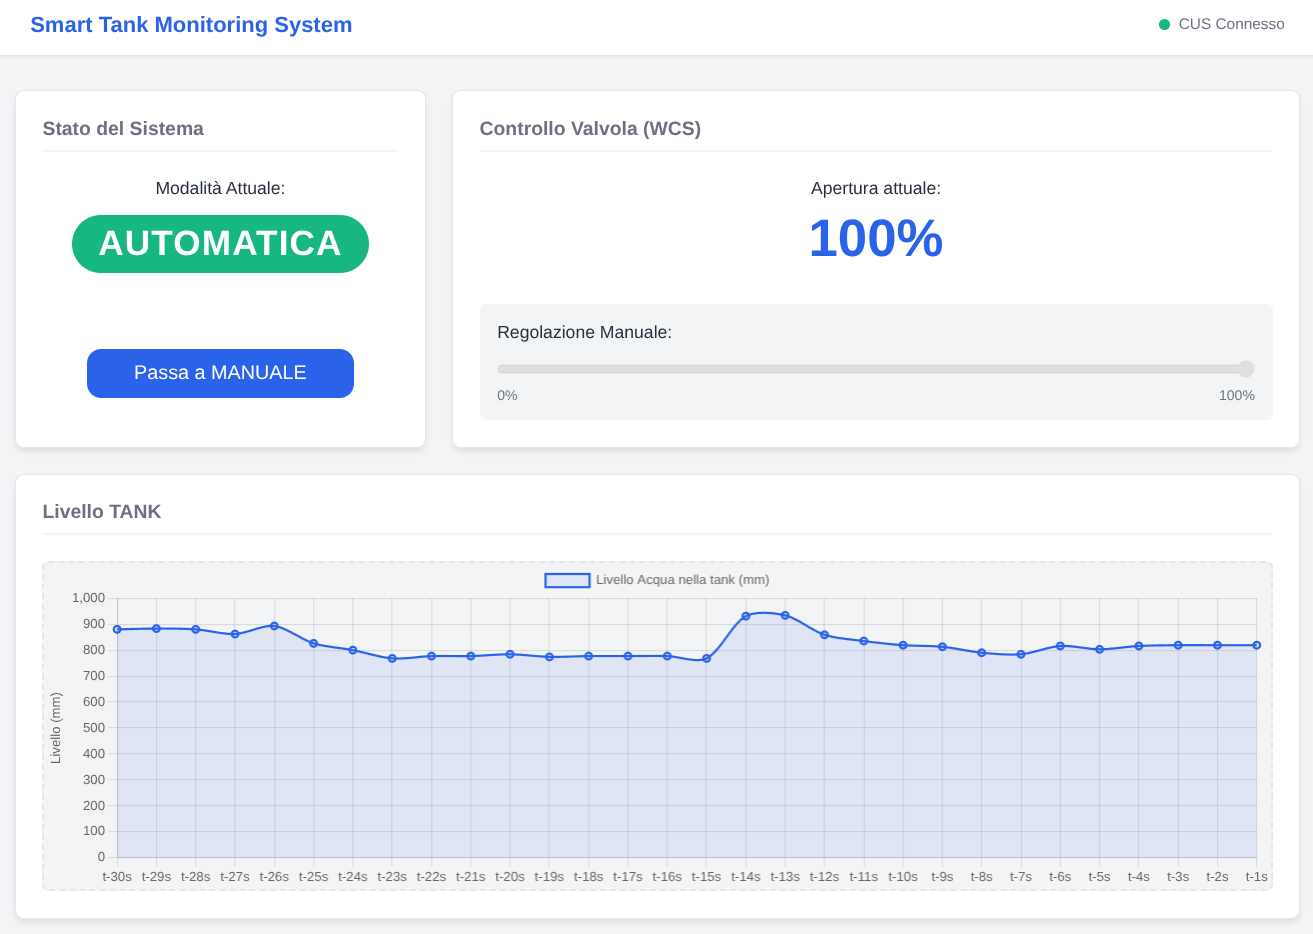
\includegraphics[width=1\textwidth]{images/dbs.png}
	\caption{Sito web del \texttt{DBS}}
	\label{fig:dbs}
\end{figure}
\newpage

\section{Protocolli di Comunicazione}

\subsection{TMS verso CUS (MQTT)}
Il TMS pubblica sul topic \texttt{tms/level} un messaggio testuale nel formato \texttt{level:\#<valore>}, dove il valore rappresenta il livello misurato in millimetri.\\
Il valore indica l'altezza in \textbf{mm} del livello dell'acqua in una cisterna da \texttt{1 metro}.

\subsection{CUS e WCS (Seriale, 115200 baud)}
Lo scambio avviene tramite messaggi testuali terminati da \texttt{\textbackslash n}, ciascuno formato da un prefisso seguito da due punti e da un valore.
\begin{table}[H]
	\centering
	\small
	\begin{tabularx}{\textwidth}{|l|p{3cm}|X|}
		\hline
		\textbf{Prefisso} & \textbf{Formato} & \textbf{Descrizione} \\
		\hline
		\texttt{mode:} & \texttt{mode:AUTO} \newline \texttt{mode:MANUAL} & Cambio di modalità, scambiato in entrambe le direzioni. \\
		\hline
		\texttt{open:} & \texttt{open:<0-100>} & Apertura valvola, scambiato in entrambe le direzioni. \\
		\hline
		\texttt{net:} & \texttt{net:OK} \newline \texttt{net:LOST} & Il CUS informa il WCS sullo stato del collegamento con il TMS. \\
		\hline
	\end{tabularx}
	\caption{Messaggi scambiati tra CUS e WCS}
\end{table}

\subsection{CUS e DBS (HTTP)}
\begin{table}[H]
	\centering
	\small
	\begin{tabularx}{\textwidth}{|l|p{3cm}|X|}
		\hline
		\textbf{Endpoint} & \textbf{Metodo} & \textbf{Descrizione} \\
		\hline
		\texttt{/api/data} & GET & Restituisce lo stato corrente del sistema: modalità, apertura valvola e storico dei livelli. \\
		\hline
		\texttt{/api/data} & POST & Riceve modalità e/o apertura da applicare. Risponde con \texttt{409} se il sistema è in \texttt{UNCONNECTED}. \\
		\hline
	\end{tabularx}
	\caption{API REST esposta dal CUS al DBS}
\end{table}

\end{document}